\subsection{\texorpdfstring{$\met$}{MET}}
\label{subsec:obj_met}

The missing transverse energy ($\met$) is computed from the negative vector sum of momenta over all PF-candidates. The ``Type-1'' correction is applied, which accounts for the JEC.

Differences in the calorimeter response to hadronic activity between simulation and data accounts for much of the difference in $\met$ scale and resolution between MC and data. A residual correction to $\met$ can be derived by calibrating the response and resolution of the hadronic recoil using $\Zjets$ and $\gamma+$jets events data \cite{recoil}. The distributions of the recoil components (parallel and perpendicular to the boson $\pt$ direction) are fit and subsequently polynomials are fit to the extracted mean and width of the recoil distributions as functions of the boson $\pt$. The mean resolutions of the parallel and perpendicular components are shown in Fig.~\ref{fig:met_MR}.


\begin{figure}[htbp]
\centering
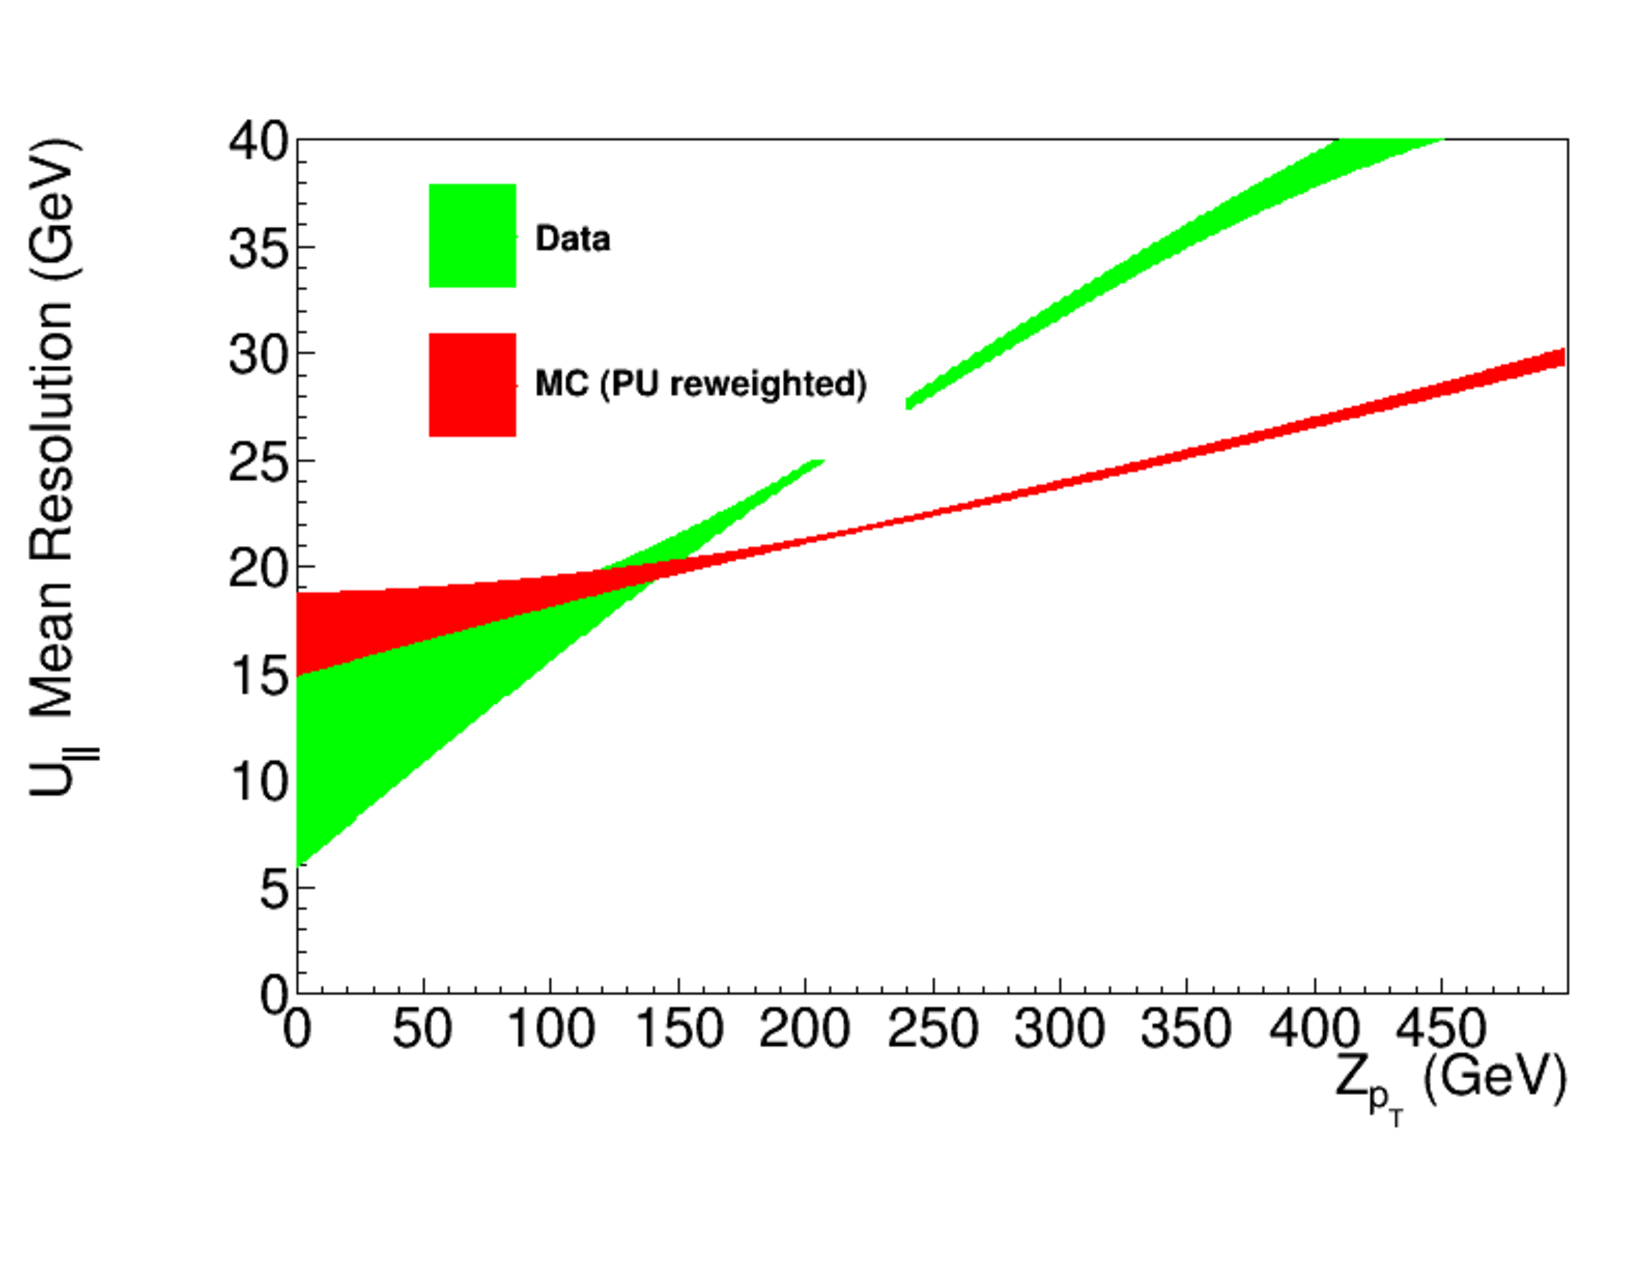
\includegraphics[width=0.48\textwidth]{figures/u1MR.pdf}
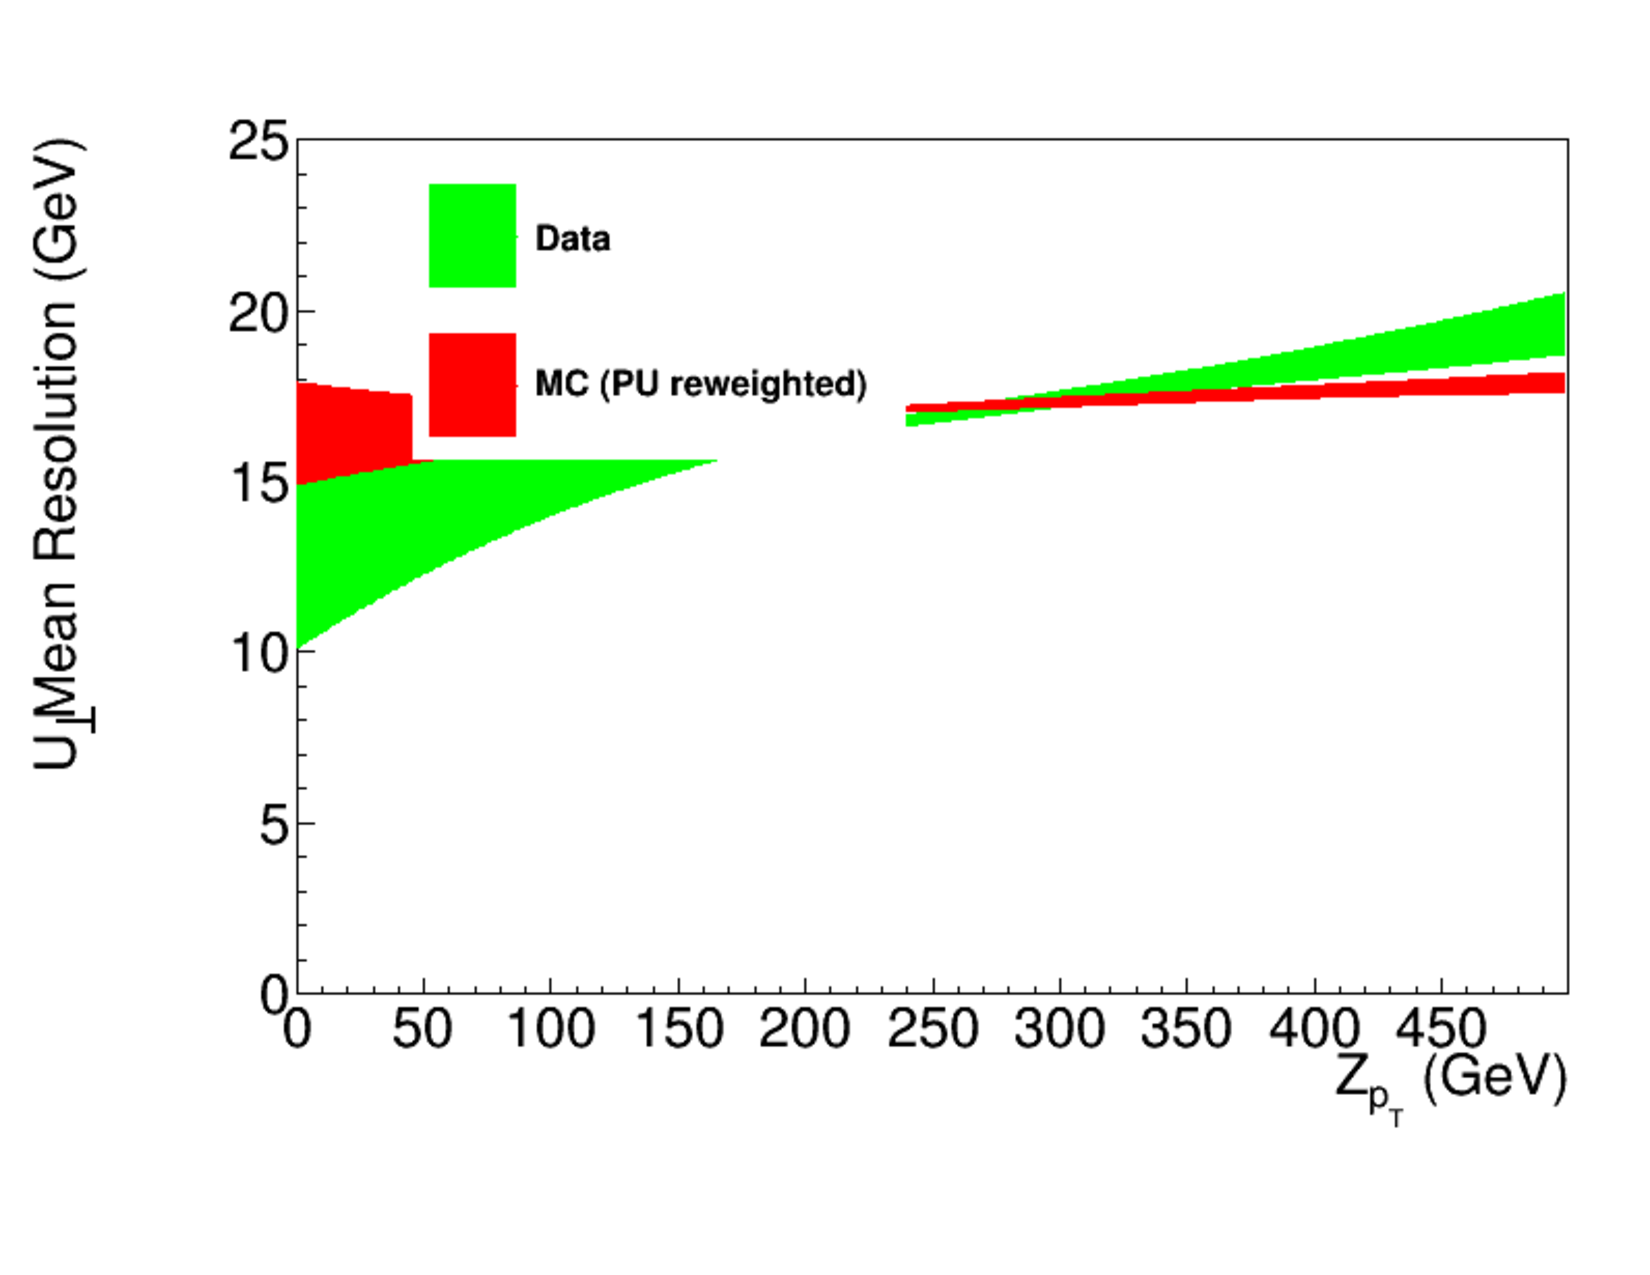
\includegraphics[width=0.48\textwidth]{figures/u2MR.pdf}
\caption{Mean resolution of hadronic recoil components that are parallel (left) and perpendicular (right) to boson $\pt$ in $\Zjets$ and $\gamma+$jets data and MC events.}
\label{fig:met_MR}.
\end{figure}


